\chapter{Introduction}

The field of autonomous driving agents has rapidly increased in modern car manufacturing. Current research topic rises the agents from parking or lane keeping assistant fully autonomous driving agents obeying the traffic rules and having the ability to react to the volatile environment in a reasonable way.

For that machine learning techniques have proven themselves as an essential part. But in order to fulfil the security standards and create a sophisticated agent it has to be trained on hundred-thousands of scenarios each having a large set of data attached, for example sensor and camera data.
The approach of \textit{Convolutional Neural Networks} (CNNs) have been proven to be powerful enough to handle such many training iterations with a huge number of input variables, while maintaining the large learning capacity. \cite{krizhevsky2012imagenet}

A CNN, as explained in \Cref{sec:CNN}, has a general structure, but can be altered to fit into the approach in various ways influencing the result. Therefore we introduce in \Cref{sec: Deep Learning Approaches} the three main approaches of using a CNN.

Further in \Cref{sec: DLL} we see that there is the need of specific languages for the design and implementation of such agents. Two languages will be discussed and compared based on their suitability regarding the \alexnet, stated in  \Cref{subsec: AlexNet}.

\section{Neural Networks}

The \nns are a construct adapted from biological processes. The general construct is very simple, but the expressiveness is very high but still not fully researched.
A neural net is made out of neurons and has one very basic function:
It takes a fixed number $n \in \mathbb{N}$ of the incoming values $x_i$ and multiplies them each with a specific weight $w_i$, where $0 \le i \le n$.
Also every neuron contains a bias $b$, which is a general value subtracted from the sum, so $\sum_{i=0}^{n} (x_i \cdot w_i) -b$. 
Often one applies an activation function to fix the value between 0 and 1. Such a function would be for example the sigmoid function or the ReLu. Without such a normalizing function the change in one neuron, which is very important could be very small compared to other values, which are not so important.
\todo{better example\\}
This new value gets forwarded to the neurons of the next layer.

Those neurons are ordered in different groups often called layers, as seen in \Cref{fig: Simple NN}.
\begin{enumerate}
	\item input layer (green):\\ \label{item input layer}
		This layer gets fed with the input values of the problem, which can be for example sensor data or pixel color values.
	\item hidden layer (blue):\\\label{item hidden layer}
		The hidden layer consists of neurons receiving the values from the previous layer, while not being obliged to have the same number of neurons (c.f. \Cref{fig: Simple NN}).
		Different hidden layer architectures can be distinguished to be deep (c.f. \Cref{fig: Deep Neural Net}). This means, that there are multiple layers of neurons within the hidden layer itself.\\
		Also a variation within the hidden layer is the possibility of fully connectivity (c.f. \Cref{fig: not fullyconnected Neural Net}). Thus some neurons don't forward their value to every neuron of the next layer.\\
		There is no rule of how to construct the best hidden layer, considering number of sub-layers, neurons per layer or the connectivity.
	\item output layer (yellow):\label{item output layer}
		The output neurons contain the value the \nn produces. Depending on the \nns purpose it can be for example a confidence value of a classification, like recognizing a stop sign, or the value of changing the steering wheel angle. 
\end{enumerate}

In order to train a \nn one has to define the behaviour the \nn should have. In an image classification example one should know what the correct class of a given image of a sign is, i.e. a speed limit sign.\\
A \nn can then be trained by giving it values for the input layer and comparing the values of the output layer with the solutions it should have resulted in. The difference can then be checked. Such a difference can be simply \texttt{true}/\texttt{false} or a value indicating how big the difference is. In the example of signs a classification of a ``speed limit 70''-sign as ``speed limit 50''-sign is still wrong, but as bad as a classification as a ``stop''-sign.\\
Using this difference value the \nn can use linear algebra algorithms to adjust the weights $w_i$ and biases $b$ to improve the output iteratively.

For further information about the underlying training algorithms please see %TODO

\todo{training ref\\}
\begin{figure}
	\centering
	\tikzset{input/.style = {ellipse,draw,fill=green!50!white, initial, initial text =}}
	\tikzset{hidden/.style = {ellipse,draw,fill=blue!50!white}}
	\tikzset{output/.style = {ellipse,draw,fill=yellow!50!white}}
	\begin{subfigure}[b]{0.25\textwidth}
	\begin{tikzpicture}[node distance = .5cm, on grid,auto]		
		\node[input] (i1) {};
		\node[input, below = of i1] (i2) {};
		\node[input, below = of i2] (i3) {};
		
		\node[hidden, above right = .25cm and 1cm of i1] (h1) {};
		\node[hidden, below = of h1] (h2) {};
		\node[hidden, below = of h2] (h3) {};
		\node[hidden, below = of h3] (h4) {};
		
		\node[output , right = 1cm of h2] (o1) {};
		\node[output , below = of o1] (o2) {};
		\coordinate[right = of o1] (c1) {};
		\coordinate[right = of o2] (c2) {};
		
		\path[->] (i1.east) edge (h1.west)
					(i1.east) edge (h2.west)
					(i1.east) edge (h3.west)
					(i1.east) edge (h4.west);
		\path[->] (i2.east) edge (h1.west)
					(i2.east) edge (h2.west)
					(i2.east) edge (h3.west)
					(i2.east) edge (h4.west);
		\path[->] (i3.east) edge (h1.west)
					(i3.east) edge (h2.west)
					(i3.east) edge (h3.west)
					(i3.east) edge (h4.west);
		\path[->] (h1.east) edge (o1.west)
				  (h2.east) edge (o1.west)
				  (h3.east) edge (o1.west)
				  (h4.east) edge (o1.west);
		\path[->] (h1.east) edge (o2.west)
					(h2.east) edge (o2.west)
					(h3.east) edge (o2.west)
					(h4.east) edge (o2.west);
		\path[->] (o1) edge (c1)
				  (o2) edge (c2);		
	\end{tikzpicture}	
	\caption{}
	\label{fig: Simple NN}
	\end{subfigure}
	\begin{subfigure}[b]{0.40\textwidth}
	\begin{tikzpicture}[node distance = .5cm, on grid,auto]		
	\node[input] (i1) {};
	\node[input, below = of i1] (i2) {};
	\node[input, below = of i2] (i3) {};
	
	\node[hidden, above right = .25cm and 1cm of i1] (h11) {};
	\node[hidden, below = of h11] (h21) {};
	\node[hidden, below = of h21] (h31) {};
	\node[hidden, below = of h31] (h41) {};
	
	\node[hidden, above right = .5cm and 1cm of h11] (h12) {};
	\node[hidden, below = of h12] (h22) {};
	\node[hidden, below = of h22] (h32) {};
	\node[hidden, below = of h32] (h42) {};
	\node[hidden, below = of h42] (h52) {};
	\node[hidden, below = of h52] (h62) {};
	
	\node[right =0.5cm of h12] (d1) {\dots};
	\node[below = of d1] (d2) {\dots};
	\node[below = of d2] (d3) {\dots};
	\node[below = of d3] (d4) {\dots};
	\node[below = of d4] (d5) {\dots};
	\node[below = of d5] (d6) {\dots};
	
	\node[hidden, right = 0.5cm of d1] (h13) {};
	\node[hidden, below = of h13] (h23) {};
	\node[hidden, below = of h23] (h33) {};
	\node[hidden, below = of h33] (h43) {};
	\node[hidden, below = of h43] (h53) {};
	\node[hidden, below = of h53] (h63) {};
	
	\node[output , right = 1cm of h33] (o1) {};
	\node[output , below = of o1] (o2) {};
	\coordinate[right = of o2] (c1) {};
	\coordinate[right = of o1] (c1) {};
	
	\path[->] (i1.east) edge (h11.west)
				(i1.east) edge (h21.west)
				(i1.east) edge (h31.west)
				(i1.east) edge (h41.west);
	\path[->] (i2.east) edge (h11.west)
				(i2.east) edge (h21.west)
				(i2.east) edge (h31.west)
				(i2.east) edge (h41.west);
	\path[->] (i3.east) edge (h11.west)
				(i3.east) edge (h21.west)
				(i3.east) edge (h31.west)
				(i3.east) edge (h41.west);
	\path[->] (h11.east) edge (h12.west)			
				(h11.east) edge (h22.west)
				(h11.east) edge (h32.west)
				(h11.east) edge (h42.west)
				(h11.east) edge (h52.west)
				(h11.east) edge (h62.west);
	\path[->] (h21.east) edge (h12.west)			
				(h21.east) edge (h22.west)
				(h21.east) edge (h32.west)
				(h21.east) edge (h42.west)
				(h21.east) edge (h52.west)
				(h21.east) edge (h62.west);
	\path[->] (h31.east) edge (h12.west)			
				(h31.east) edge (h22.west)
				(h31.east) edge (h32.west)
				(h31.east) edge (h42.west)
				(h31.east) edge (h52.west)
				(h31.east) edge (h62.west);			
	\path[->] (h41.east) edge (h12.west)			
				(h41.east) edge (h22.west)
				(h41.east) edge (h32.west)
				(h41.east) edge (h42.west)
				(h41.east) edge (h52.west)
				(h41.east) edge (h62.west);
					
	\path[->] (h13.east) edge (o1.west)
				(h23.east) edge (o1.west)
				(h33.east) edge (o1.west)
				(h43.east) edge (o1.west)
				(h53.east) edge (o1.west)
				(h63.east) edge (o1.west);		
	\path[->] (h13.east) edge (o2.west)
				(h23.east) edge (o2.west)
				(h33.east) edge (o2.west)
				(h43.east) edge (o2.west)
				(h53.east) edge (o2.west)
				(h63.east) edge (o2.west);		
	\end{tikzpicture}
	\caption{}
	\label{fig: Deep Neural Net}
	\end{subfigure}	
	\begin{subfigure}[b]{0.32\textwidth}
		\begin{tikzpicture}[node distance = .5cm, on grid,auto]		
		\node[input] (i1) {};
		\node[input, below = of i1] (i2) {};
		\node[input, below = of i2] (i3) {};
		
		\node[hidden, above right = .25cm and 1cm of i1] (h11) {};
		\node[hidden, below = of h11] (h21) {};
		\node[hidden, below = of h21] (h31) {};
		\node[hidden, below = of h31] (h41) {};
		
		\node[hidden, above right = .5cm and 1cm of h11] (h12) {};
		\node[hidden, below = of h12] (h22) {};
		\node[hidden, below = of h22] (h32) {};
		\node[hidden, below = of h32] (h42) {};
		\node[hidden, below = of h42] (h52) {};
		\node[hidden, below = of h52] (h62) {};
		
		
		\node[output , right = 1cm of h32] (o1) {};
		\node[output , below = of o1] (o2) {};
		\coordinate[right = of o2] (c1) {};
		\coordinate[right = of o1] (c1) {};
		
		\path[->] (i1.east) edge (h11.west)
			(i1.east) edge (h21.west)
			(i1.east) edge (h31.west)
			(i1.east) edge (h41.west);
		\path[->] (i2.east) edge (h11.west)
			(i2.east) edge (h21.west)
			(i2.east) edge (h31.west)
			(i2.east) edge (h41.west);
		\path[->] (i3.east) edge (h11.west)
			(i3.east) edge (h21.west)
			(i3.east) edge (h41.west);

		\path[->] (h11.east) edge (h12.west)			
			(h11.east) edge (h22.west)
			(h11.east) edge (h32.west);
		\path[->] (h21.east) edge (h22.west)
			(h21.east) edge (h32.west)
			(h21.east) edge (h42.west)
			(h21.east) edge (h12.west);
		\path[->] (h31.east) edge (h32.west)
			(h31.east) edge (h42.west)
			(h31.east) edge (h52.west)
			(h31.east) edge (h62.west);			
		\path[->] (h41.east) edge (h42.west)
			(h41.east) edge (h52.west)
			(h41.east) edge (h62.west);
		\path[->] (h12.east) edge (o1.west)
			(h22.east) edge (o1.west)
			(h52.east) edge (o1.west)
			(h62.east) edge (o1.west);		
		\path[->] (h12.east) edge (o2.west)
			(h22.east) edge (o2.west)
			(h32.east) edge (o2.west)
			(h42.east) edge (o2.west)
			(h52.east) edge (o2.west)
			(h62.east) edge (o2.west);		
		\end{tikzpicture}
		\caption{}
		\label{fig: not fullyconnected Neural Net}
	\end{subfigure}
	% das Dritte ist wenig Sinvoll vom Aufbau her
\end{figure}


\section{Convolutional Neural Network (CNN)}\label{sec:CNN}

A CNN is a special class of deep feed-forward \nns. On of the main design goals of a CNN is that they require a minimal amount of preprocessing. This is an important aspect, because they are often fed with images. Preprocessing high resolution images is very costly in terms of computational time. In the context of autonomous driving the time is even more crucial, since the driving agent needs to be able to react to spontaneous events.

Like most parts of \nns, also the CNNs are inspired by biological processes. It is mainly based on the connectivity pattern of an animals visual cortex, where special neurons respond only to stimuli of their receptive field, represented as rectangles lying in the image. Partially overlapping guarantees a complete coverage of the field of view. \cite{wiki:CNN}
These separation into those receptive fields has also the advantage that is reduces the effort to train a CNN. The weights and biases of neurons of each receptive field are equal. This is reasonable since for example a speed limit road sign should be identified independent whether it is located next to the road, like on a normal road, or above the road, like on an highway. %TODO: ref

Further CNNs make strong and mostly correct assumptions about the nature of images, like stationary of statistics and locality of pixel dependencies. This leads to fewer connections and parameters, compared to a normal feed-forward neural net with similar sized layers, and therefore reduces the time it takes to be trained, while being only slightly worse in their best-performance. \cite{krizhevsky2012imagenet}


\subsection{AlexNet} \label{subsec: AlexNet}

The \textit{\alexnet} is on of the best performing CNN architectures currently known. It is trained on the ImageNet subsets of \texttt{ILSVRC-2010} and \texttt{ILSVRC-2012}\footnote{Further information: http://www.image-net.org/challenges/LSVRC/} and became famous because of its result being way ahead of all other competitors.

A highly optimized GPU implementation of this architecture combined with innovative features is publicly available. Those features lead to improve performance and reduce training time.
An important note is that the original test is dated back to 2012 and therefore was used with an overall GPU memory of 6GB, with which training took abound six days. With modern hardware the training can be done faster, or the model can be trained much more. \cite{krizhevsky2012imagenet}

\todo{maybe calc the possible speed up based on ``Hardware for Machine Learning''}

\begin{figure}[ht]
	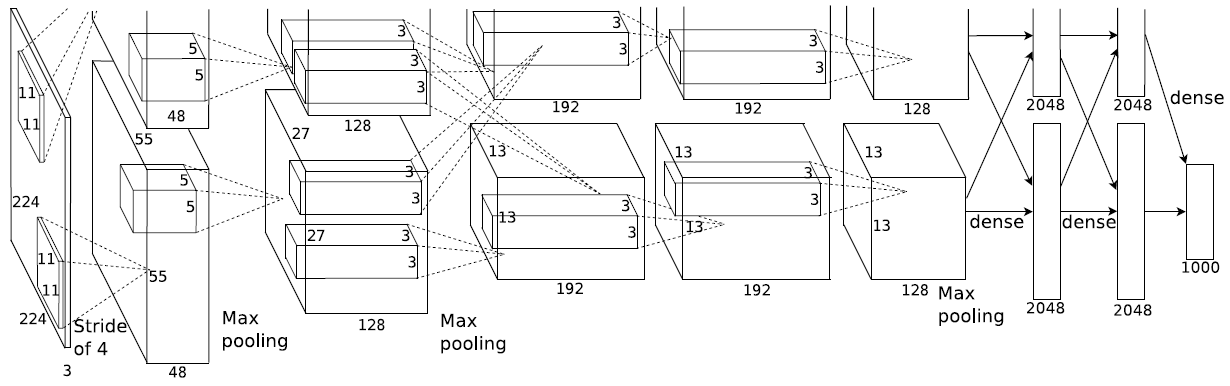
\includegraphics[scale = 0.5]{src/pic/AlexNet-structure.PNG}
	\caption{The \alexnet-architecture for two GPUs. It consists of 5 convolutional layers (at the beginning) and three fully-connected layers (at the end). The GPUs only communicate between two layers, but never within a layer.\cite{krizhevsky2012imagenet}}
	\label{pic: AlexNet}
	\todo{Vereinfachen der Zeichnung\\}
\end{figure}

\section{Available Deep Learning Approaches}\label{sec: Deep Learning Approaches}

There are various approaches of autonomous driving agents making a variety of assumptions and differ in numerous options. But they can be mostly categorized into two major groups of approaches: mediated perception approaches and behavior reflex approaches. \cite{chen2015deepdriving}

In this paper we further analyze a suggested third group, called direct perception, which can traced to \cite{gibson1979ecological} in the mid 50's, but was sharply criticized by researchers of the other two groups, i.e. in \cite{ullman1980against}. %TODO: fix 60's to be the first

All these three groups differ in the way of interpreting the given sensor data and whether or not to create a some what bigger picture based on consequent data.

\subsection{Mediated Perception} \label{subsec: Mediated Perception}

The mediated perception approach is a multi-component continuous process. Every component recognizes specific aspects for driving. For example traffic signs, lanes, other cars. Those components are then combined into one single world state representing the cars surrounding based on the sensor data. \cite{KITTI}\\
These world states are 3D models of the current world. Cars are identified using a classifier and then often surrounded by a 3D bounding box. An example can be seen in \Cref{pic: 3D Bounding Box}. By comparing different frames generated one can estimate the speed and distance to those objects and derive an A.I. based precedence behavior. \cite{KITTI}\cite{chen2015deepdriving}

The often stated problems with such approaches are, that computing such a scene is costly in terms of computation time. Some information is irrelevant, redundant or even misleading due to inaccuracy of sensors. To perform a right turn the sensor information of the distance to a car left behind me is irrelevant, but becomes very important when taking a left turn.\\
Additionally many of the subtasks are still open research topics themselves. For example a reliable lane detection throughout various weather conditions or even a new road not having any drawn lines yet. \cite{aly2008real}\\
Also mediated perception approaches require very detailed information up front, like up-to-date maps.

The approach of mediated perception is a reasonable and very sturdy way of handling such a complex task, but has its drawbacks regarding computational time and additional knowledge.

\begin{figure}
	\centering
	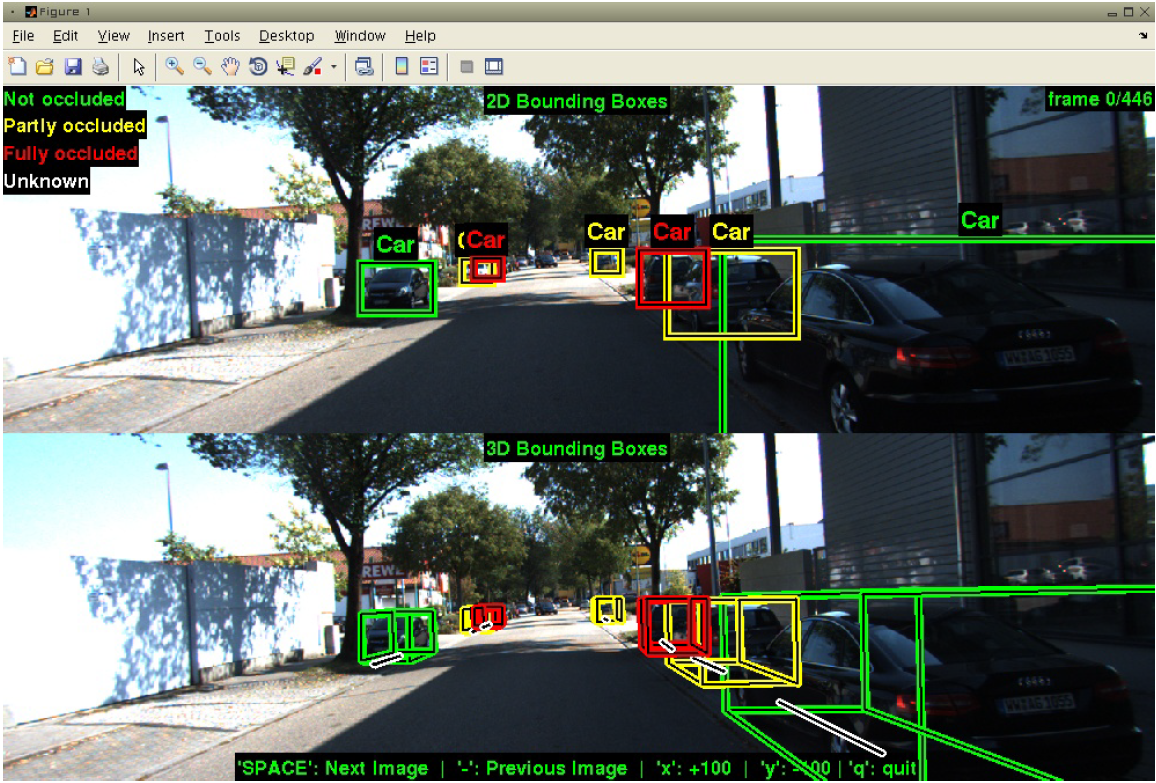
\includegraphics[scale=0.4]{src/pic/3D-boundingbox-example.png}
	\caption{An example of a scene using 3D bounding boxes. This image is taken from the MATLAB delvopment kit of \cite{KITTI}}
	\label{pic: 3D Bounding Box}
\end{figure}

\subsection{Behavior Reflex}\label{subsec: Behavior Reflex}

The behavior reflex approach of constructing a reliable autonomous driving agent can be dated back to 1989 , where researchers tried to directly map a single frame to a decision of a steering angle. For such approaches a quite simple \nn were created. \\
The network \alvinn, shown in \Cref{pic: ALVINN}, consisted of a single hidden layer, used back-propagation and is fed by two cameras: a $30\times32$ pixel video and a $8\times32$ pixel range finder retina. The input neurons fired depending on the blue color band of its pixel, because it is believed to infer the highest contrast between road and non-road. The difference in color of road and non-road was fed back to the network. The bias (activation level) is proportional to the proximity of the corresponding area, based on the likelihood and importance of having road in particular fields of the image.\cite{pomerleau1989alvinn}\\
For example having recognized that the road abruptly ends right in front of the car is more important than recognizing that there is a road in the top left corner.\\

Such systems, even though they are simple compared to the in \Cref{subsec: Mediated Perception} mentioned mediated perception approaches, have been proven to have the capability to perform simple tasks. It can elegantly be trained by having a human drive a car with the cameras equipped and forward the images to the \nn and adding the current steering angles as a label.\cite{chen2015deepdriving}\\

The problem with behavior reflex approaches is, that they reach their limits very early when adding more complex scenarios. Having simple alternations to the trained scenarios, which enforce a different behavior, is very hard to train to such a \nn.\\
For example comparing a simple straight 3 lane road with the car in the middle, as sketched in \Cref{fig: behavior sketches}. The system is confidently able to hold the angle and make small adjustments to stay in the lane (\Cref{fig: behavior sketches: free lane}). But what if on the same road there is an other car in the middle lane in front of the agent, which is slower? Having quite the same input the system would have to overtake the car left or right (considering an american highway) (\Cref{fig: behavior sketches: blocked lane}). Now also considering a car in front, which has the same speed. One can simple stay in the lane (\Cref{fig: behavior sketches: shared lane}). This maneuver is very hard to train to a simple \nn like \alvinn.

\todo{noch mehr?\\}

\begin{figure}
	\centering	
	\tikzset{->,very thick,>=stealth}
	\begin{subfigure}[b]{0.32\textwidth}
		\begin{tikzpicture}[scale=0.9] % left picture
		\newcommand{\lineLength}{0.75}
		\newcommand{\lineSpace}{0.5}
		\newcommand{\startSpace}{0.25}
		
		\fill[green!50!black] (0,0) rectangle (5,5);		% background
		\fill[gray!50!black] (0.5,0) rectangle (4.5,5);     % pavement
		\fill[yellow!75!black] (0.55,0) rectangle (0.6,5);  % left yellow line
		\fill[yellow!75!black] (4.4,0) rectangle (4.45,5);  % right yellow line
		
		% left lane breaks		
		\fill[white] (1.84,\startSpace) rectangle (1.86,\lineLength+\startSpace);		
		\fill[white] (1.84,1*\lineLength + 1*\lineSpace + \startSpace) rectangle (1.86,2*\lineLength + 1*\lineSpace + \startSpace);
		\fill[white] (1.84,2*\lineLength + 2*\lineSpace + \startSpace) rectangle (1.86,3*\lineLength + 2*\lineSpace + \startSpace);
		\fill[white] (1.84,3*\lineLength + 3*\lineSpace + \startSpace) rectangle (1.86,4*\lineLength + 3*\lineSpace + \startSpace);
		
		% right line breaks
		\fill[white] (3.12,\startSpace) rectangle (3.14,\lineLength+\startSpace);		
		\fill[white] (3.12,1*\lineLength + 1*\lineSpace + \startSpace) rectangle (3.14,2*\lineLength + 1*\lineSpace + \startSpace);
		\fill[white] (3.12,2*\lineLength + 2*\lineSpace + \startSpace) rectangle (3.14,3*\lineLength + 2*\lineSpace + \startSpace);
		\fill[white] (3.12,3*\lineLength + 3*\lineSpace + \startSpace) rectangle (3.14,4*\lineLength + 3*\lineSpace + \startSpace);
		
		% cars
		\fill[red] (2.1,0.2) rectangle (2.1 + 0.8,0.2 + 1.5);
		\draw[->,very thick,  color = white] (2.5,0.4) -- (2.5,1.5);
		\draw[->,very thick,  color = green!75!black] (2.5,2) -- (2.5,3);
		
		%		\node [trapezium, minimum width = 3.6cm, trapezium angle=25,rotate = 180, opacity = 0.4, color = gray!50!white, fill] at (2.5,2) (test) {};
		%		\fill[gray!50!white, opacity = 0.4] (0.5,2.378) rectangle (4.5,5);
		\end{tikzpicture}
		\caption{free lane}
		\label{fig: behavior sketches: free lane}
	\end{subfigure}
	\begin{subfigure}[b]{0.32\textwidth}
		\begin{tikzpicture}[scale=0.9] % middle picture
		\newcommand{\lineLength}{0.75}
		\newcommand{\lineSpace}{0.5}
		\newcommand{\startSpace}{0.25}
		
		\fill[green!50!black] (0,0) rectangle (5,5);		% background
		\fill[gray!50!black] (0.5,0) rectangle (4.5,5);     % pavement
		\fill[yellow!75!black] (0.55,0) rectangle (0.6,5);  % left yellow line
		\fill[yellow!75!black] (4.4,0) rectangle (4.45,5);  % right yellow line
		
		% left lane breaks		
		\fill[white] (1.84,\startSpace) rectangle (1.86,\lineLength+\startSpace);		
		\fill[white] (1.84,1*\lineLength + 1*\lineSpace + \startSpace) rectangle (1.86,2*\lineLength + 1*\lineSpace + \startSpace);
		\fill[white] (1.84,2*\lineLength + 2*\lineSpace + \startSpace) rectangle (1.86,3*\lineLength + 2*\lineSpace + \startSpace);
		\fill[white] (1.84,3*\lineLength + 3*\lineSpace + \startSpace) rectangle (1.86,4*\lineLength + 3*\lineSpace + \startSpace);
		
		% right line breaks
		\fill[white] (3.12,\startSpace) rectangle (3.14,\lineLength+\startSpace);		
		\fill[white] (3.12,1*\lineLength + 1*\lineSpace + \startSpace) rectangle (3.14,2*\lineLength + 1*\lineSpace + \startSpace);
		\fill[white] (3.12,2*\lineLength + 2*\lineSpace + \startSpace) rectangle (3.14,3*\lineLength + 2*\lineSpace + \startSpace);
		\fill[white] (3.12,3*\lineLength + 3*\lineSpace + \startSpace) rectangle (3.14,4*\lineLength + 3*\lineSpace + \startSpace);
		
		% cars
		\fill[red] (2.1,0.2) rectangle (2.1 + 0.8,0.2 + 1.5);	% agent
		\draw[->,very thick,  color = white] (2.5,0.4) -- (2.5,1.5);
		\draw[->,very thick,  color = green!75!black] (2,1.8) -- (1.3,2.5) -- (1.3,3);
		\draw[->,very thick,  color = green!75!black] (3,1.8) -- (3.8,2.5) -- (3.8,3);
		
		
		\fill[orange] (2.1,3.2) rectangle (2.1 + 0.8,3.2 + 1.5);	% other car
		\draw[->,very thick,  color = white] (2.5,3.4) -- (2.5,4);
		\end{tikzpicture}
		\caption{slower car in the same lane}
		\label{fig: behavior sketches: blocked lane}
	\end{subfigure}
	\begin{subfigure}[b]{0.32\textwidth}
		\begin{tikzpicture}[scale=0.9] % right picture
		\newcommand{\lineLength}{0.75}
		\newcommand{\lineSpace}{0.5}
		\newcommand{\startSpace}{0.25}
		
		\fill[green!50!black] (0,0) rectangle (5,5);		% background
		\fill[gray!50!black] (0.5,0) rectangle (4.5,5);     % pavement
		\fill[yellow!75!black] (0.55,0) rectangle (0.6,5);  % left yellow line
		\fill[yellow!75!black] (4.4,0) rectangle (4.45,5);  % right yellow line
		
		% left lane breaks		
		\fill[white] (1.84,\startSpace) rectangle (1.86,\lineLength+\startSpace);		
		\fill[white] (1.84,1*\lineLength + 1*\lineSpace + \startSpace) rectangle (1.86,2*\lineLength + 1*\lineSpace + \startSpace);
		\fill[white] (1.84,2*\lineLength + 2*\lineSpace + \startSpace) rectangle (1.86,3*\lineLength + 2*\lineSpace + \startSpace);
		\fill[white] (1.84,3*\lineLength + 3*\lineSpace + \startSpace) rectangle (1.86,4*\lineLength + 3*\lineSpace + \startSpace);
		
		% right line breaks
		\fill[white] (3.12,\startSpace) rectangle (3.14,\lineLength+\startSpace);		
		\fill[white] (3.12,1*\lineLength + 1*\lineSpace + \startSpace) rectangle (3.14,2*\lineLength + 1*\lineSpace + \startSpace);
		\fill[white] (3.12,2*\lineLength + 2*\lineSpace + \startSpace) rectangle (3.14,3*\lineLength + 2*\lineSpace + \startSpace);
		\fill[white] (3.12,3*\lineLength + 3*\lineSpace + \startSpace) rectangle (3.14,4*\lineLength + 3*\lineSpace + \startSpace);
		
		% cars
		\fill[red] (2.1,0.2) rectangle (2.1 + 0.8,0.2 + 1.5);
		\draw[->,very thick,  color = white] (2.5,0.4) -- (2.5,1.5);
		\draw[->,very thick,  color = green!75!black] (2.5,2) -- (2.5,3);
		
		\fill[orange] (2.1,3.2) rectangle (2.1 + 0.8,3.2 + 1.5);	% other car
		\draw[->,very thick,  color = white] (2.5,3.4) -- (2.5,4.5);
		\end{tikzpicture}
		\caption{equal fast car in same lane}
		\label{fig: behavior sketches: shared lane}
	\end{subfigure}
	\caption{The 3 scenarios causing problems with behavior reflex approaches. The red block is the agent, the orange block the other car, the white arrows indicate the velocity and the green arrows the logically deduced behaviors.}
	\label{fig: problematic behavior sketches}
\end{figure}

\begin{figure}
	\centering
	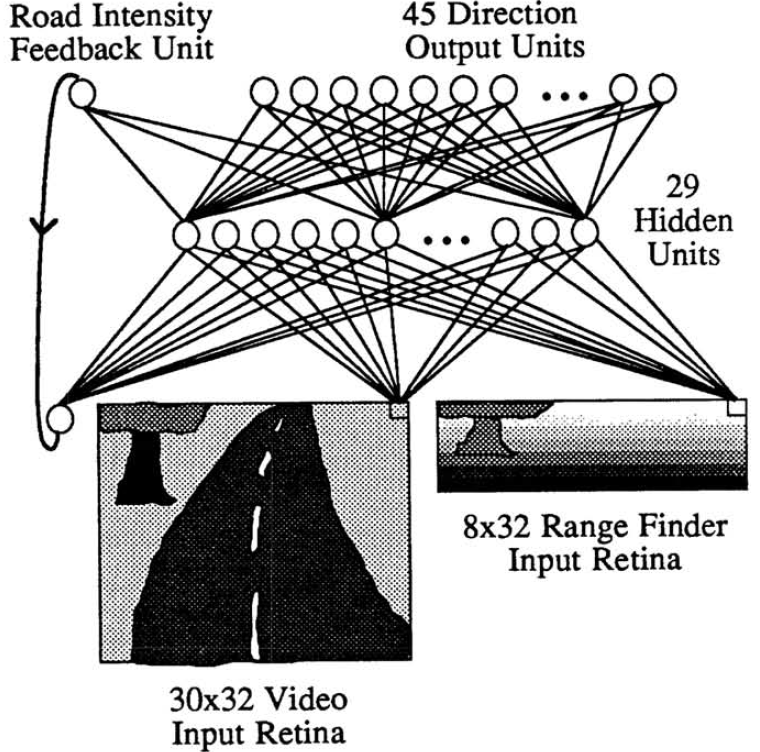
\includegraphics[scale=0.4]{src/pic/ALVINN.png}
	\caption{The \nn called \alvinn and used as a behavior reflex based autonomous agent. \cite{pomerleau1989alvinn}}
	\label{pic: ALVINN}
\end{figure}

\subsection{Direct Perception}\label{subsec: Direct Perception}

%In this paper we further analyze a suggested third group, called direct perception, which can traced to \cite{gibson2014ecological} in the late 80's, but was sharply criticized by researchers of the other two groups, i.e. in \cite{ullman1980against}.

The direct perception is the third group of approaches, which can be dated back to the 1954 and was mainly researched by James J. Gibson. \cite{gibson1954theory} The approach is based on analyzing a picture not simply deducing a steering angle, or velocity change, like the behavior reflex approaches (cf. \Cref{subsec: Behavior Reflex}), but also performing further computation without parsing it into a 3D world state model like the mediated perception approaches (cf. \Cref{subsec: Mediated Perception}). \cite{chen2015deepdriving}\\
So it is a third paradigm, which can be interpreted as a hybrid of the two other paradigms. The approach tries to identify only the meaningful affordance indicators and make a decision based on those parameters. 

We further consider a design based on \cite{chen2015deepdriving} and their way of training.

\todo{\begin{enumerate}
\item how to learn the affordance
\item how to conclude affordance to action
\end{enumerate}}

\section{Deep Learning Languages}\label{sec: DLL}
\todo{\begin{enumerate}
\item why need a language
\item what should it in general do?
\item state that different languages ex.
\end{enumerate}}

\subsection{CNNArchLang}\label{subsec: CNNArch}

(The whole description is based on\cite{CNNArch})

One language for modeling CNNs is CNNArchLang. This language is developed at the Chair of Software Engineering at the RWTH Aachen University and part of the MontiCar language family. 

\subsection{MxNet}\label{subsec: MxNet}

general information from \cite{chen2015mxnet}

